			    A Bitonic Sort\cite{bitonic_ref} is a comparison based parallel sorting algorithm. A random input sequence in first converted into a Bitonic sequence , which monotonically increases and then decreases thus the name Bitonic.
			    The rotations applied to a Bitonic sequence is also Bitonic.The random input is coversion to Bitonic sequence is achieved with a \textit{Bitonic-Splitter}.\newline
			    Let \[ 
				  S = \langle x_0,x_1,..x_{n-1}\rangle 
				\] be Bitonic sequence such that
				\[
				    x_0 \leq x_1 \leq ... \leq x_{n/2-1} \quad \textrm{and} \quad  x_{n/2} \leq x_{n/2+1} \leq ... \leq x_{n-1}  \quad \textrm{holds}
				\]
			    Consider the following subsequences
				\[
				  S_{1} =  \langle min(x_0,x_{n/2}), min(x_1,x_{n/2+1}),..,min(x_{n/2-1},x_{n-1})\rangle
				\]
				\[
				  S_{2} =  \langle max(x_0,x_{n/2}), max(x_1,x_{n/2+1}),..,max(x_{n/2-1},x_{n-1})\rangle
				\]
			    with the following property.
				\[
				  \forall _{x} \forall _{y}. x \in S_{1}  \wedge  y \in S_{2} \quad x < y
				\]
			    Both $S_{1}$ and $S_{2}$ are Bitonic. A sorted sequence is produced as a result of applying $S_{1}$ and $S_{2}$ recursively. The above procedure is called \textit{Bitonic Split}. Firstly \textit{Bitonic Split} is performed 
			    in the input random sequence which trasforms any given sequence to a Bitonic sequence which is then fed to the \textit{Bitonic Merge} network. The \textit{Bitonic Merge} converts the splitted sequence to sorted sequence.
			    sequence. A 16 input Bitonic sorter configuration is shown in the Figure \ref{fig:BitonicSorter16}. In our case we expand the same configuration to a 32 input sorter . The outputs $z_{0}$ to $z_{31}$  will
			    be connected to the corresponding \textit{Function-Units} with respect to the physical address.
				    \begin{figure}[!ht]
					      \includegraphics[width=\linewidth]{BitonicSorter16.png}
					    \caption{A 16 input BitonicNetwork}
				    \label{fig:BitonicSorter16}
				    \end{figure}
			    The arrow indicates a Comparator. The up-down arrow indicates an ascending comparator and the down-to up indicates a descending one. Both the comparator element configurations are shown in Figure \ref{fig:Comparators}. 
			    An N input Bitonic Network consists of $O(N.log_{2}(N)^{2})$ comparators and has a combinatorial depth of $O(log_{2}(N)^{2})$.
				    \begin{figure}[!ht]
					      \includegraphics[width=\linewidth]{Comparators.png}
					    \caption{Basic $2 x 2$ comparator elements of a Bitonic sorter}
				    \label{fig:Comparators}
				    \end{figure}
			\subsubsection{Bitonic Network as Network Router}
				  The Bitonic Network is only a sorting network, does not have enough intelligence to act it as a network router in practical cases. Everything works well when all \textit{Function-Units} 
				  are ready to send the \textit{Data-Packets} to its target. But this is not the case most of the times. Many \textit{Function-Units} can still be in a state where its outputs are not ready,
				  at the same time some of the \textit{Function-Units} are ready with their outputs. In this case Bitonic Network can fail in routing the \textit{Data-packets} to the right destinations because all
				  that are not ready can feed an unknown \textit{Target-Address}. Two solutions were identified as the following.
				  \subsubsection{Bitonic Network with Routers}
					      This is a proposed solution before realizing the Bitonic-Banyan \cite{batcher_banyan_ref}( Batcher's Banyan)  network. In this case the invalid \textit{Target-Address} problem is sorted
					      out by adding and two extra stages at the input and output of the Bitonic Sorter. At input we add an \textit{Address-Resolver} module for each comparators. In the architecture an invalid 
					      addresses\footnote{An invalid address here means when the a \textit{Function-Unit} has no outputs ready at a given point of time to send to another \textit{Function-Unit}, 
					      which can result in any address at the input of the DTN. The \textit{VALID} bit is asserted to a \textit{LOW} in every clock cycle by the \textit{Function-Unit} when not \textit{Data-Packets} are ready.}
					      is identified by a \textit{VALID} bit in the \textit{Data-Packet} (Figure \ref{fig:Data_Packet}). All \textit{Functional-Unit} writes a \textit{LOW} to the \textit{VALID} bit of its output packets in every clock cycle unless an packet is ready. 
					      In this way the network can interpret the validity of the \textit{Data-Packet} and act accordingly. The \textit{Address-Resolver} feeds the input of each comparator with a predefined hardcoded address according to the position of the comparator. 
					      Figure \ref{fig:Address_Resolver} shows a implementation of the \textit{Address-Resolver}.
					      \begin{figure}[!ht]
							\includegraphics[width=\linewidth]{Address_Resolver.png}
						      \caption{Address resolution}
					      \label{fig:Address_Resolver}
					      \end{figure}
					      The \textit{Address-Resovler} is a simple combinatorial multiplexer which switches the address based on the \textit{VALID} bit of address and is connected to all the $N$ comparators of input.
					      For an $N$ input Bitonic network the hardcoded address is defined as $N -1 + C$ , where $C$ is the position of the the comparator which ranges from $1$ to $N$. This ensures the 
					      comparators are fed with an addresses which is greater that $N -1$, which enables the sorter to work even if some of the inputs are invalid. In other words the \textit{Address-Resovler}
					      switches the input of the Bitonic network to  valid address at the instant when the \textit{VALID} bit is \textit{HIGH}. One  more problem that to be resolved
					      still is the sorted output sequence the network. The sorter will sort the \textit{Data-Packets} with all the hardcoded addresses positioned at last of the address sequence but still the actual addresses can
					      be routed into wrong destinations. For eg: If the input is an address sequence $\langle31,X_{1},X_{2},..,X_{31}\rangle$ (where $X_{i}$ indicates invalid address) which results in the sorted output sequence 
					      of $\langle31,32,33,..,63\rangle$. The routing is wrong since the $31$ is routed to target $0$. To resolve this we have to use a stage of sequencial routers at the output of the network.
					      
					      
					      The routers have forward and reverse routing path and \textit{Data-packet} is routed to either forward or reverse path based on the distance to the target. The distance to each destination is hardcoded 
					      in a routing table which enables faster decision making. The configuration is shown in Figure \ref{fig:RouterNetwork} .The drawback is a \textit{stall} signal is required
					      to stop the network to take new  \textit{Data-packets} until the old ones are delivered to the corresponding target  \textit{Function-Units}. The worst case time for a packet to reach the target
					      from the router network will be $N / 2$ .In other words in the worst case we have to stall network for $N/2$ clock cycles without doing anything useful in that time. The best
					      case would be when all the inputs are valid. Besides the circuit is sequencial and the \textit{stall} is active which degrades the DTN performance. This is because the \textit{stall} creates backpressure which
					      will be propegated to all the \textit{Function-Units} and the \textit{Control-Unit}.Also a router element is a complicated state machine which consumes considerable amount of resources when we have $32$ instances of the same. 
					      This fact lead us to use a Bitonic-Banyan\cite{batcher_banyan_ref} cascaded network which resolves this address permutation problem in constant time.
					      \begin{figure}[!ht]
							\includegraphics[width=\linewidth]{RouterNetwork.png}
						      \caption{Router Network}
					      \label{fig:RouterNetwork}
					      \end{figure}
				  \subsubsection{Bitonic-Banyan Network}
					      We utilize the self routing property of a Bitonic-Banyan\footnote{A Bitonic-Banyan cascaded network is called a Batcher-Banyan network in the reference paper\cite{batcher_banyan_ref}.
					      We call it as Bitonic-Banyan  network all over this paper to give an intuitive meaning how the network is constructed.} network \cite{batcher_banyan_ref} when the invalid 
					      \textit{Target-addresses} are found at the input. The configuration contains
					      a Bitonic Sorting Network cascaded with a Banyan routing network. As in the case of a Bitonic Network we use the $2 X 2$ switching element(comparator) but the connection state of this
					      element is determined by the destination tags of the input, in our case the \textit{Target address}. A Bitonic network is capable or realizing arbritary permutations of the inputs. 
					      But still the routing is not proper with invalid \textit{Data-packet} at the inputs. Here comes the use of Banyan network which can route the sorted outputs to appropriate
					      \textit{Target addresses}. As mentined before, special kind of modified switching elements are used which is quite differant from the configuration of normal Bitonic comparators.
					      The switching elements are added with some extra logic to route the larger target address \textit{Data-packets} to the direction pointed by the arrow. 
					      Figure \ref{fig:Batcher_Switches} depicts the switch configuration in different possible scenarios. 
					      
					      An $X$ indicates incomplete inputs. This switch basically moves all the $X$s from the input sequence to the bottom of the sequence.
					      Thus for any input sequence of Data-Packets with a set of  the invalid addresses $\{U_{0},U_{1},..,U_{r-1}\}$, the Bitonic network will produce an output sequence of $\langle A_{0},A_{1},..,A_{K},..,U,U,..,U \rangle$ , where
					      $ K = 32 - r -1$. Figure \ref{fig:Batcher_Switches} shows the modified switching element for the Bitonic network of the DTN. The \textit{Normal-Switch} is an ascending comparator which is shown in Figure \ref{fig:Comparators} and
					      the \textit{Modified-Switch} the one which is shown in Figure \ref{fig:Switching_Element}. which handles the invalid address situation.
					      \begin{figure}[!ht]
						      \includegraphics[width=\linewidth]{Batcher_Switches.png}
						      \caption{Modified switch handles different scenarios in Bitonic network}
					      \label{fig:Batcher_Switches}
					      \end{figure}
					      \begin{figure}[!ht]
						      \includegraphics[width=\linewidth]{Switching_Element.png}
						      \caption{Switching element of Bitonic network}
					      \label{fig:Switching_Element}
					      \end{figure}
					      \begin{figure}[!ht]
						      \includegraphics[width=\linewidth]{Banyan_Tree.png}
						      \caption{An 8 input Banyan network}
					      \label{fig:Banyan_Tree}
					      \end{figure}
					      The next stage is a Banyan Network which takes up the sorted sequences by the Bitonic network and route to the proper destination. Note that a shuffle permutaion is added at the input of the Banyan network.
					      This is shown in Figure \ref{fig:Banyan_Tree} for an 8 input Banyan network configuration. The input shuffle permutation is such that two destination tags (\textit{Target-Address} in our case) are different in MSB. We simply expand the same to 32. 
					      It is proven \cite{batcher_banyan_ref} that 
					      an Banyan network with a the given input shuffle permutation as shown in \ref{fig:Banyan_Tree} can completely route a sorted sequence when the incomplete inputs appear either at high end or low end of the list without any conflicts. We have already moved all the incomplete \textit{Data-Packets}
					      to the lower end of the sequence with the help of modified switch. 
					      The \textit{Data-Packets} in the Banyan network is based on the $i^{th}$ bit of the \textit{Target-Address}, where $i$ is the stage index. For an $N$ input Banyan network we have $log_{2}(N)$ 
					      stages and combinatorial circuit depth. Also a Banyan newtwork is collision free if the input sequences are sorted ascending
					      thus strongly guaranteeing the delivery of \textit{Data-Packets} at proper destination. In our case 
					      the sequence can also have invalid \textit{Data-Packets} which is in the tail of the sequence. Different scenarios in handling of incomplete input for a Banyan switch is shown in Figure \ref{fig:Banyan_Switches}.
					      A $X$ corresponds to incomplete inputs. The valid inputs are the bit position of the stage $i$ of the \textit{Target-Address}. Based on this bit the \textit{Data-packet} is routed up or down.
					      \begin{figure}[!ht]
						      \includegraphics[width=\linewidth]{Banyan_Switches.png}
						      \caption{Different scenarios in Banyan network switch }
					      \label{fig:Banyan_Switches}
					      \end{figure}
					      It has also verified with benchmarks \cite{sorting_network_on_fpgas} that for $N > 8$ the latency due to combinatorial depth of a Bitonic network is more that when it is piplelined. So we have implemented 5 stage pipleline 
					      for th Bitonic network and a 5 stage for the Banyan network.Altogether for the SCAD arhitecture the synchronous \textit{Bitonic-Banyan} version of DTN is shown in Figure \ref{fig:Batcher_Banyan_Combined}.
					      \begin{figure}[!ht]
						      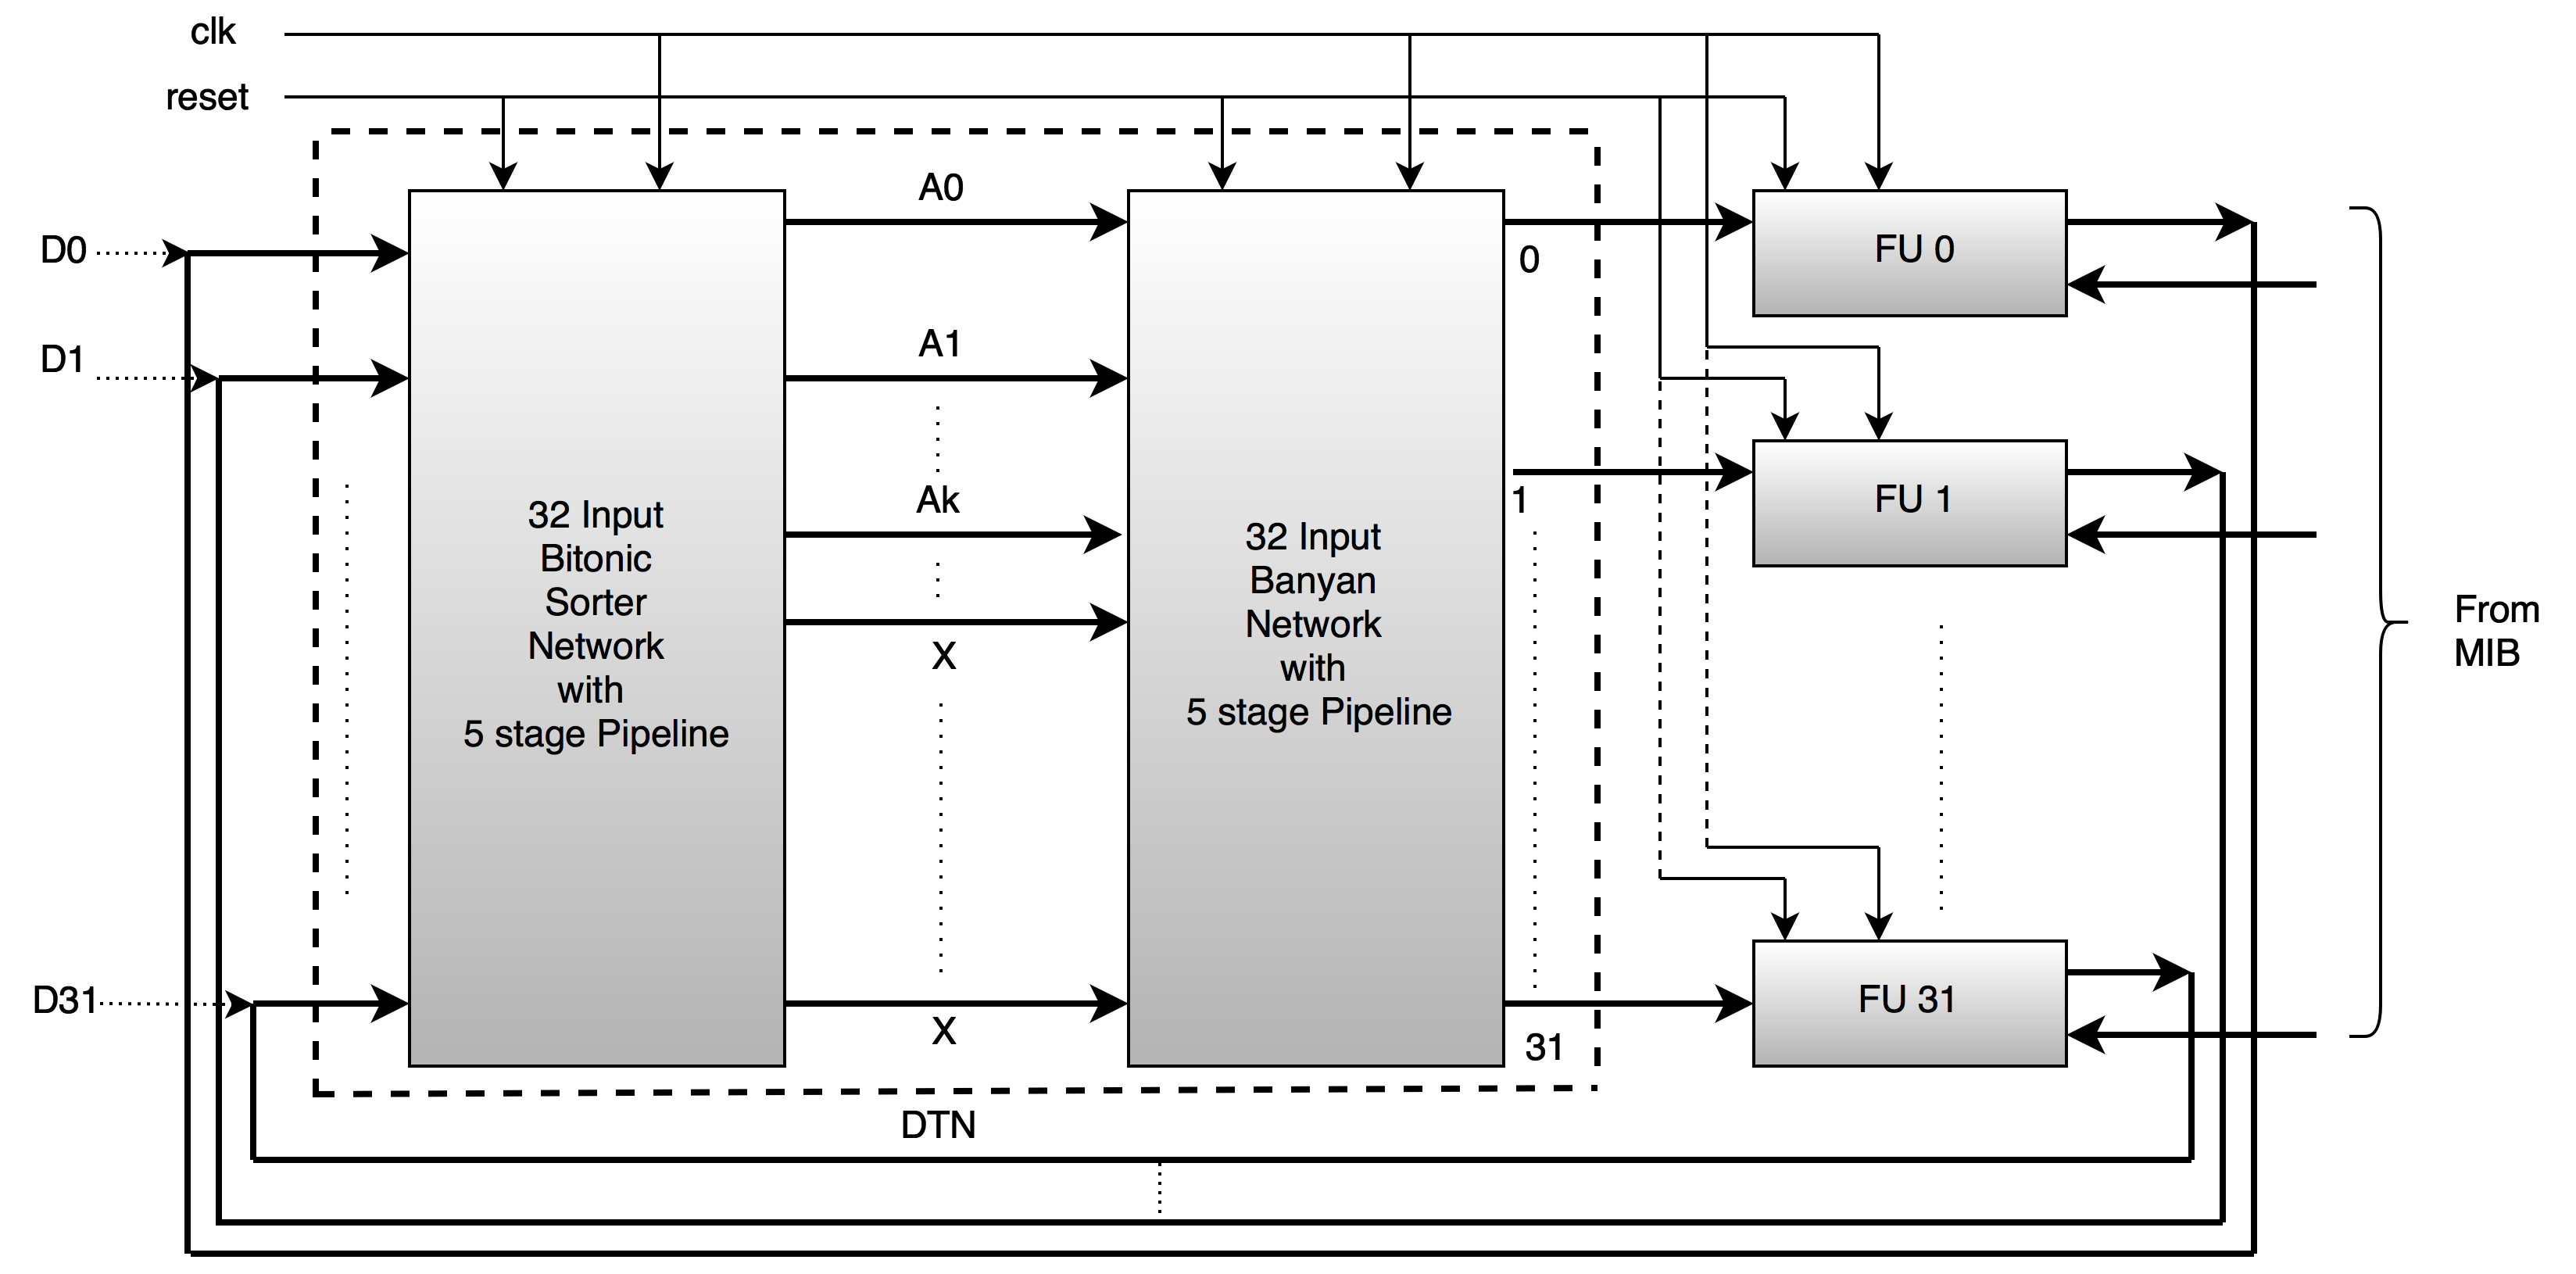
\includegraphics[width=\linewidth]{Batcher_Banyan_Combined.png}
						      \caption{DTN of SCAD arhitecture with Bitonic-Banyan network}
					      \label{fig:Batcher_Banyan_Combined}
					      \end{figure}
				 \subsubsection{Resource utilization}
					      The resource ulitzation on the FPGA shows significant advantage on Bitonic-Banyan over the sequencial implementation with routers. The table \ref{fig:bitonic_utilisation}
					      shows a comparison table for both the implementation. It is clear to see that the Bitonic-Banyan consumes not much than a the sequencial version , but still has benifit in
					      terms of constant time in delivering \textit{Data-Packets} to its destination.
					    \begin{table}
					    \begin{center}
					      \begin{tabular}{l | c | c }
						\textbf{Site Type}  & \textbf{Bitonic with routers (\%)} & \textbf{Bitonic-Banyan (\%)} \\
						\hline \hline
						Slice LUTs 			& 30.85 & 37.65 \\ 
						\quad LUT as Logic		& 30.85 & 37.65 \\
						\quad LUT as Memory		& 0.00 & 0.00 	\\
						Slice Registers 		& 11.12	& 13.53 \\
						\quad Register as Flip Flop	& 11.12	& 13.53	\\
						\quad Register as Latch	& 0.00	& 0.00	\\
						F7 Muxes			& 0.00	& 0.00	\\
						F8 Muxes 			& 0.00	& 0.00	\\
					      \end{tabular}
					      \end{center}
					      \caption{Resource utilization of DTN with Bitonic network}
					      \label{fig:bitonic_utilisation}
					    \end{table}


